\section{Graphical Models [24pts]}

In the Kingdom of Westeros, Summer has come. Jon Snow, the King in the North, has taken the responsibility to defeat the Giants and protect the realm.

If Jon Snow can get Queen Cersei and Daenerys Queen of the Dragons to help him Jon is likely to beat the giants. Cersei and Daenerys are powerful women who are skeptical of the existence of Giants and will most likely only consider joining Jon if the are shown evidence of an imminent Giant attack. They can only be shown of an attack if Jon captures a live Giant.

The Bayesian network that represents the relationship between the events described above is shown below. Use the following notation for your variables: Jon Snow captures a live Giant ($X_1$), Jon shows Censei and Daenerys a live Giant  ($X_2$), Cersei agrees to help ($X_3$), Daenerys agrees to help ($X_4$) and Giants defeated ($X_5$).
\begin{figure}[!hbtp]
\centering
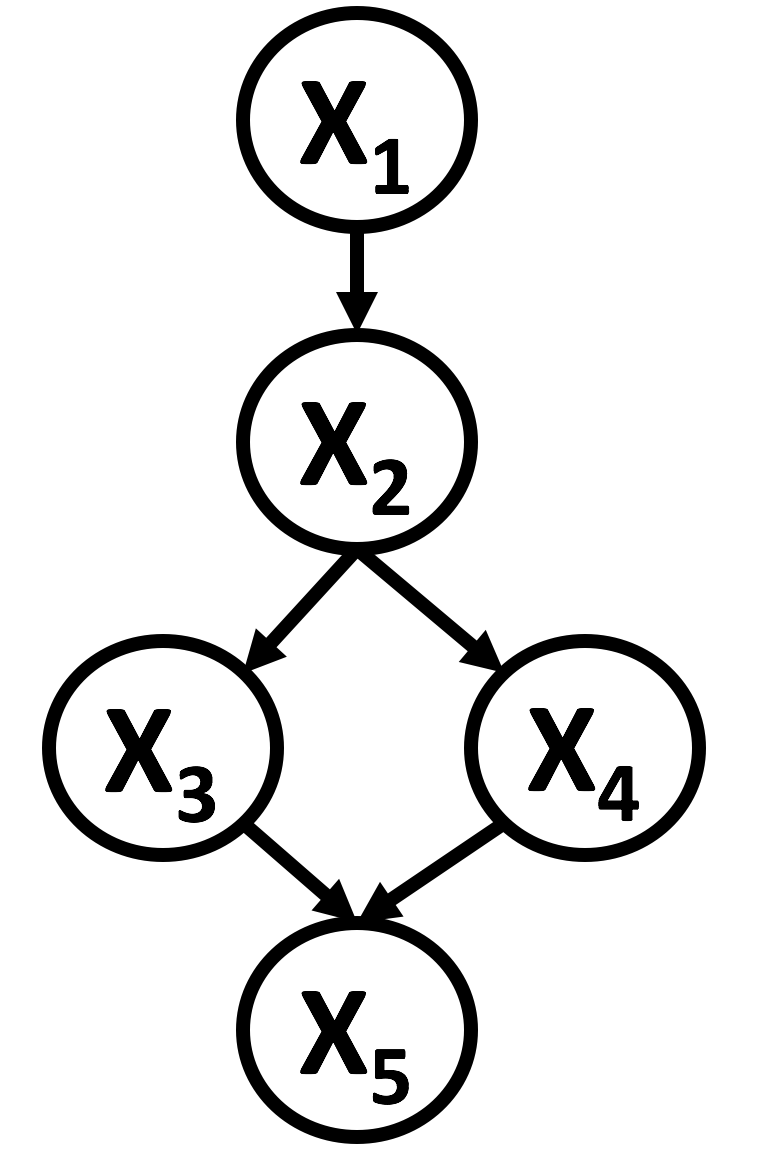
\includegraphics[scale=0.3]{figures/q2.png}
\end{figure}

\begin{enumerate}
\item \textbf{[3pt]} Write down the factorization of the above directed graphical model.

\begin{tcolorbox}[fit,height=1cm, width=15cm, blank, borderline={1pt}{-2pt},nobeforeafter]
%solution
\end{tcolorbox}


\item \textbf{[3pt]} Each random variable represented in the above Bayesian network is binary valued (i.e. either the event happens or it does not). State the minimum number of parameters you need to fully specify  this Bayesian network.

\begin{tcolorbox}[fit,height=1cm, width=2cm, blank, borderline={1pt}{-2pt},nobeforeafter]
%solution
\end{tcolorbox}


\item \textbf{[3pt]} If we didn't use these conditional independence assumptions above, what would be the minimum number of parameters we would need to model any joint distribution over the same set of random variables?

\begin{tcolorbox}[fit,height=1cm, width=2cm, blank, borderline={1pt}{-2pt},nobeforeafter]
%solution
\end{tcolorbox}



\item \textbf{[10pts]} For the following questions fill in the blank with the smallest set $\mathcal{S}$ of random variables needed to be conditioned on in order for the independence assumption to hold. For example $X_i \perp X_j \mid \mathcal{S}$. What is the smallest set $\mathcal{S}$ that makes this statement true? The empty set $\emptyset$ is a valid answer, additionally if the independence assumption cannot be satisfied no matter what we condition on then your answer should be 'Not possible'.
\begin{enumerate}

\item \textbf{[2pt]} $X_1 \perp X_3 \mid $ \begin{tcolorbox}[fit,height=1cm, width=2cm, blank, borderline={1pt}{-2pt},nobeforeafter]
%solution 
\end{tcolorbox}  \\

\item \textbf{[2pt]} $X_1 \perp X_5 \mid$ \begin{tcolorbox}[fit,height=1cm, width=2cm, blank, borderline={1pt}{-2pt},nobeforeafter]
%solution 
\end{tcolorbox}   \\

\item \textbf{[2pt]} $X_2 \perp X_4 \mid $ \begin{tcolorbox}[fit,height=1cm, width=2cm, blank, borderline={1pt}{-2pt},nobeforeafter]
%solution 
\end{tcolorbox}  \\

\item \textbf{[2pt]} $X_3 \perp X_4 \mid $ \begin{tcolorbox}[fit,height=1cm, width=2cm, blank, borderline={1pt}{-2pt},nobeforeafter]
%solution 
\end{tcolorbox}  \\

\item \textbf{[2pt]} $X_2 \perp X_5 \mid $ \begin{tcolorbox}[fit,height=1cm, width=2cm, blank, borderline={1pt}{-2pt},nobeforeafter]
%solution 
\end{tcolorbox}  \\

\end{enumerate}

\clearpage
\item \textbf{[5pts]} Jon gets his friend Sam to calculate some estimates of his chances. Sam returns to Jon with the following conditional probabilities tables:

\begin{table}[H]
    \centering
    \begin{tabular}{|c|c|}
    \hline
         $X_1=0$ & $0.3$  \\ \hline
         $X_1=1$ & $0.7$    \\  \hline
    \end{tabular}
    \\ 
    \begin{tabular}{|c|c|c|}
    \hline
            & $X_1=0$ & $X_1=1$   \\  \hline
        $X_2=0$ & $0.8$ & $0.25$ \\  \hline
        $X_2=1$ & $0.2$  & $0.75$    \\  \hline
    \end{tabular}
    \\ 
    \begin{tabular}{|c|c|c|}
    \hline
            & $X_2=0$ & $X_2=1$   \\  \hline
        $X_3=0$ & $0.5$ & $0.6$ \\  \hline
        $X_3=1$ & $0.5$  & $0.4$    \\  \hline
    \end{tabular}
    \\ 
    \begin{tabular}{|c|c|c|}
    \hline
            & $X_2=0$ & $X_2=1$   \\  \hline
        $X_4=0$ & $0.3$ & $0.2$ \\  \hline
        $X_4=1$ & $0.7$  & $0.8$    \\  \hline
    \end{tabular}
    \\ 
    \begin{tabular}{|c|c|c|c|c|}
    \hline
            & $X_3=0, X_4=0$ & $X_3=0,X_4=1$ & $X_3=1,X_4=0$ & $X_4=1,X_3=1$   \\  \hline
        $X_5=0$ & $0.4$ & $0.7$ & $0.8$ & $0.5$ \\  \hline
        $X_5=1$ & $0.6$  & $0.3$ & $0.2$ & $0.5$    \\  \hline
    \end{tabular}
    \caption{Sam's Conditional Probability tables}
\end{table}

Using the conditional probabilities for our graphical model, compute the following (Your answers should be given to 5 decimal places): 
\begin{enumerate}
\item \textbf{[2pts]} $P(X_1=0, X_2=1, X_3=0, X_4=1, X_5=0)$. 


\begin{tcolorbox}[fit,height=1cm, width=4cm, blank, borderline={1pt}{-2pt},nobeforeafter]
%solution 
\end{tcolorbox}\\


\item \textbf{[3pts]}$P(X_1 = 1 | X_3 = 1)$ 

\begin{tcolorbox}[fit,height=1cm, width=4cm, blank, borderline={1pt}{-2pt},nobeforeafter]
%solution 
\end{tcolorbox}\\

\end{enumerate}
\end{enumerate}

\newpage
